% Subsection 4.2: detection  -*- LaTeX -*-

\subsection{Detection}
\label{Detection}

The object detection and characterization code lies in its own namespace, \code{lsst::detection}.

\subsubsection{C++ Classes}

Detection contains the framework classes related to processing astronomical images.
The fundamental objects are:
\begin{itemize}
\item Source detection
  \begin{itemize}
  \item \code{Threshold}:
    A threshold level.
  \item \code{Footprint}:
    A set of pixels (internally stored as \code{Span}s).
  \item \code{DetectionSet}:
    An STL collection of \code{Footprint}s associated
    with a \code{MaskedImage} (\Sec{FW}).
  \end{itemize}
  
\item Source measurement
  \begin{itemize}
  \item \code{MeasurePixProcFunc}, \code{Measure}:
    Classes designed to measure the properties
    of \code{DiaSource}s.
  \item \code{Peak}:
    A peak in an image.
  \end{itemize}
  
\item Miscellaneous
  \begin{itemize}
  \item \code{BCircle}:
    A description of a circular disk.
  \end{itemize}
  
\item Classes ready for DC3 (\ticket{322})
  \begin{itemize}
  \item \code{PSF}, \code{dgPSF}:
    Place-holders to describe point spread functions.
  \item \code{Defect}:
    A CCD defect, such as a bad column.
  \end{itemize}
\end{itemize}

All of these classes were implemented for DC2, and make use of
the support classes defined in mwi (e.g.~\code{mwi::data::LsstBase},
\code{mwi::utils::Trace}).  They are documented using doxygen,
although the level of the documentation is patchy;  in particular
high level documentation (motivation and examples) tends to be missing.

\paragraph{Source detection}

\subparagraph{Footprint}
The fundamental class in source detection is a \code{Footprint}, a set
of connected pixels above (or below) some threshold. Two pixels are
said to be `connected' if they touch along a side or by a corner.  The
internal representation of a \code{Footprint} is an STL container of
\code{Span}s --- a triple of a row number in the image and a starting
and ending column.\footnote{We are currently schizophrenic as to
  whether such ranges are inclusive or exclusive; \code{Span}s are
  inclusive, while e.g.~\code{vw::BBox2i} is exclusive. We need
  to be consistent in DC3 and beyond.}
The user currently needs to be aware of this; for
DC3 we should provide an iterator over the pixels in a \code{Footprint},
and possibly move \code{Footprint} to \code{fw} (\Sec{FW}).

The threshold defining a \code{Footprint} is a class in its own right,
imaginatively named \code{Threshold}, which may be implicitly
initialised from a numerical value or constructed to be a negative
value (which \code{Footprint}s must lie below), and/or a value
in units of an image's variance or standard deviation.

In DC2 we have been detecting in an unsmoothed image, and demanding
at least a certain number of pixels above/below a threshold.  In general
we wish to search for objects based on a maximum likelihood
analysis of the image;  in the limit of faint sources with
uncorrelated Gaussian noise, this corresponds to smoothing the
image with the assumed shape of the sought-for source (e.g.~with
the PSF).  We have not implemented any such scheme for DC2,
although the machinery is present in \code{fw}'s \code{Kernel}
classes.  The natural generalisation of this approach is to
search in a $\chi^2$ image.  Another question is the actual
value of the threshold to adopt, but this (although an interesting
question) has little impact upon the image processing algorithms
employed.

A \code{Footprint} or set of \code{Footprint}s only makes sense
in the context of an image;  a \code{DetectionSet} associates
an STL container of \code{Footprint}s with a \code{MaskedImage},
and may be constructed from the \code{MaskedImage} and a \code{Threshold};
it is templated over the \code{Image} and \code{Mask} pixel types.

Experience with other surveys has shown that \code{Footprint}s provide
a natural representation of sources;  if the pixel intensities are
stored within the class, a \code{Footprint} may be used to define
a source, even if two or more sources overlap.  We may expect that
\code{Footprint}s will acquire more methods as LSST DM proceeds.


\paragraph{Source measurement}

DC2 only concerns itself with difference imaging, and thus with
\code{DiaSource} (\Sec{FW}).  The current implementation of the source
measurement code uses a functor scheme (class
\code{MeasurePixProcFunc} driven by \code{Measure}) similar to that
used for iterating over \code{Image}s.  This seems appropriate,
certainly for the simple moments that we are measuring in DC2. A
suitable generalisation, possibly iterating over \code{Footprint}s,
should be used in DC3.

\subparagraph{Peak}
An approach to defining object identity is to determine the set
of peaks present in a set of images;  in order to treat blended
sources simultaneously --- as well as to cull noise peaks --- it
is often convenient to treat all peaks present in a \code{Footprint}
together.  The class \code{Peak} was defined to fill this r\^ole,
although it has not been employed in DC2.  

\subsubsection{Classes ready for DC3 (\ticket{322})}

Some functionality is present in the DC2 code base,
although not used in the DC2 processing.

\subparagraph{Interpolation over defects}
A CCD defect, such as a bad column, is described by a \code{Defect};
the list of problems for a given CCD can be read from a \code{Policy}
(\Sec{Policy}) file.  Once identified, and given some information
about the PSF,  these defects are interpolated over using linear
predictive coding (LPC), and labelled as interpolated in the
associated \code{Mask}.  This patching over defects avoids problems with
e.g.~cosmic ray detection code which otherwise detects all bad columns;
it is of course possible to write more complicated algorithms that
handle bad pixels, but it's simpler to interpolate them away.

\subparagraph{PSFs}
We have classes \code{PSF} and \code{dgPSF} (a double-Gaussian
inheriting from \code{PSF}) to describe the PSF.  These are
present purely as placeholders, and to give the \code{Defect}
and cosmic ray code a measure of the seeing.

\subparagraph{Cosmic Rays}
LSST expects to perform cosmic ray (CR) splits, but not all datasets
allow such luxuries, and it is often advantageous to be able to
detect CRs in a single band --- for example, if the two exposures
need to be aligned before CR removal can be attempted.  The current
implementation is based on that used by SDSS and looks for gradients
in the image that exceed the band limit (i.e.~are sharper than
the PSF).  The algorithm seems to work reasonably well on the
Megacam data used in DC2, but may well need work or replacement
for DC3.

\begin{figure}[htbp]
  \begin{center}
    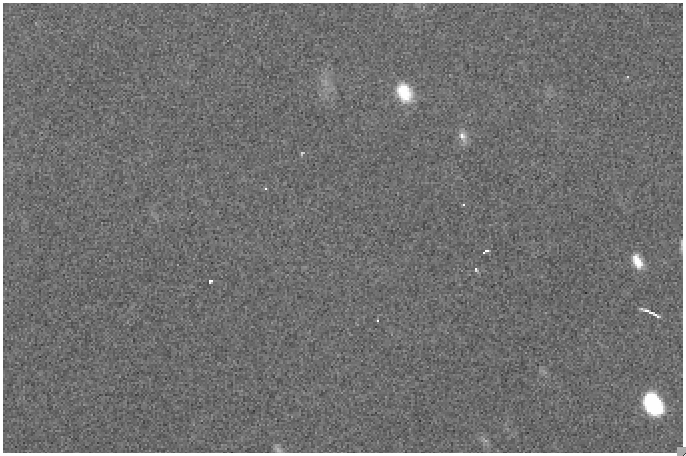
\includegraphics[height=60mm,angle=90]{figures/CR-before}
    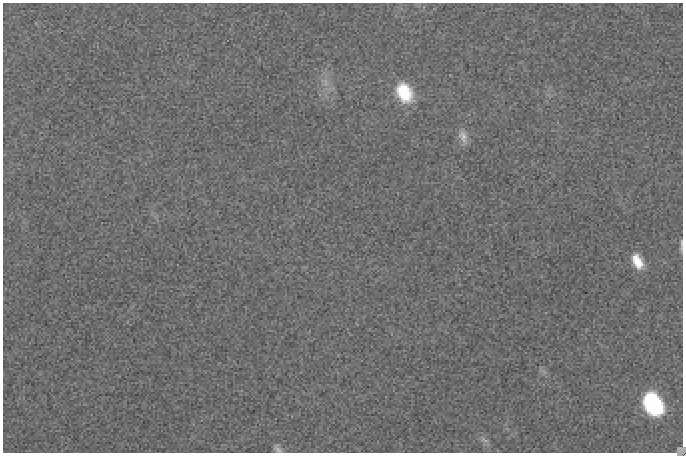
\includegraphics[height=60mm,angle=90]{figures/CR-after}
  \end{center}
\caption{A $343\times228$ pixel portion of a CFHT image (\code{cal-53535-i-797722\_1})
  before (left) and after (right) defect and cosmic ray interpolation. The entire
  $2k\times4k$ image contains approximately 1100 cosmic rays.
}
\label{FigCRbefore}
\end{figure}
